%%%%%%%%%%%%%%%%%%%%%%%%%%%%%%%%%%%%%%%%%%%%%%%%%%%%%%%%%%%%%%%%%%%%%%%%%%%%
%% Trim Size: 9.75in x 6.5in
%% Text Area: 8in (include Runningheads) x 5in
%% ws-ijait.tex   :   01-10-2014
%% Tex file to use with ws-ijait.cls written in Latex2E.
%% The content, structure, format and layout of this style file is the
%% property of World Scientific Publishing Co. Pte. Ltd.
%%%%%%%%%%%%%%%%%%%%%%%%%%%%%%%%%%%%%%%%%%%%%%%%%%%%%%%%%%%%%%%%%%%%%%%%%%%%
%%

\documentclass{ws-ijait}
\usepackage[superscript]{cite}
\usepackage{multirow}
\begin{document}

\markboth{Jagdish Chakole, Nachiket Doddamani, Manish Kurhekar}
{Unleashing the Power of Deep Learning: A Performance Comparison of LSTM, GRU, CNN, and Transformer Models ...}


%%%%%%%%%%%%%%%%%%%%% Publisher's Area please ignore %%%%%%%%%%%%%%%
%
\catchline{}{}{}{}{}
%
%%%%%%%%%%%%%%%%%%%%%%%%%%%%%%%%%%%%%%%%%%%%%%%%%%%%%%%%%%%%%%%%%%%%

\title{Unleashing the Power of Deep Learning: A Performance Comparison of LSTM, GRU, CNN, and Transformer Models in Non Ferrous Metal Price Forecasting on the London Metal Exchange}

\author{Jagdish Chakole\footnote{jchakole@iiitn.ac.in},\hspace{0.2cm}Nachiket Doddamani \footnote{nachiketdoddamani@gmail.com}}

\address{Department of Computer Science and Engineering, \\Indian Institute of Information Technology,\\
 Nagpur, Maharashtra 441108,
India}



\author{Manish Kurhekar}

\address{Department of Computer Science and Engineering, \\Visvesvaraya National Institute of Technology,\\
	Nagpur, Maharashtra 440010,
	India\\
	manishkurhekar@cse.vnit.ac.in}

\maketitle

\begin{history}
\received{(Day Month Year)}
\revised{(Day Month Year)}
\accepted{(Day Month Year)}
%\comby{(xxxxxxxxxx)}
\end{history}

\begin{abstract}
Metals, particularly non-ferrous metals, play a pivotal role as raw materials in numerous industries, serving as essential components for a nation's industrial and economic growth. The fluctuating prices of these metals pose a significant challenge for industries aiming to procure them at optimal costs. While various approaches, including machine learning, have been employed for metal price prediction, there remains room for improvement in the accuracy and efficiency of these models. Notably, recent advancements in deep learning have demonstrated impressive performance. This research delves into the application of state-of-the-art deep learning models tailored for sequential data to enhance the prediction accuracy of metal prices. The main contribution of this research work is the use of the Transformer model to predict metal price and its comparison with the state-of-the-art deep learning models tailored for sequential data.  Through empirical studies, we explore the efficacy of prominent deep learning architectures, including Long Short-Term Memory (LSTM), Gated Recurrent Unit (GRU), Convolutional Neural Network (CNN), and Transformer models. The objective is to discern the model that exhibits superior performance in capturing the intricate patterns and temporal dynamics inherent in metal price time series data. By leveraging these advanced techniques, our research aims to contribute to the refinement of predictive models for optimizing metal procurement strategies. Our experimental results show that the proposed Transformer-based model outperformed the LSTM, GRU, and CNN base model to predict the non-ferrous metal prices including Aluminium, Copper, Zinc, and Nickel.
\end{abstract}

\keywords{Non-ferrous metals, Deep Learning, Transformer, London Metal Exchange.}

\section{Introduction}
Metals are the basic raw materials for many industries. Many metals are used to manufacture machines for diverse sectors like agriculture, automobile, construction, and more. Almost all industries directly or indirectly depend upon metals. So, the price of the finished product depends on the metals, that are required as raw materials to a product or as raw materials to equipment required to manufacture the product. The price of the metals depends on many diverse factors including demand and supply of the metal, geopolitical situation, etc. The price of the metals fluctuates over time. One of the objectives of the industry is to purchase metals at an optimal price as the price of their finished product is based on raw materials price. Governments and industries are in need to know the future price of these metals for decision-making.
\par The motivation for this work is related to the advancement in computer technology and the Data Science domain and its ubiquitous use. The majority of the global stock and commodity exchanges are working online because of the technological advancements. Historical and current trading data like price action, and volume data is easily available at affordable cost in electronic form \cite{chakole2023tutorial}. The performance of data-driven machine learning and deep learning methods has improved significantly. The availability of models and clean datasets have the potential to predict future prices or trends.
\par In this research work, we are interested in predicting the future price of non-ferrous metals as it is significant for the growth and development of the country. We are specifically interested in non-ferrous metals, as these metals are mostly useful in manufacturing industries because of their significant properties \cite{watkins2004econometric}. Non-ferrous metals are non-magnetic and non-iron based metals like Aluminium, Copper, Zinc, Nickel, etc.
\par The main contribution of this research work is twofold, The first is a model based on Transformer to predict metal price. Till now no other work has used a Transformer model to predict non-ferrous metal price. Second, we have compared the performance of the proposed model with the state-of-the-art deep learning model for sequential data.
\par The time series dataset for the daily prices of non-ferrous metals exhibits a consistent time difference between consecutive data points, rendering it a sequential data format. Similarly, Natural Language Processing (NLP) data also follows a sequential structure. Recently, there has been a notable surge in the development of deep learning-based predictive models for sequential data within the NLP domain, demonstrating noteworthy performance. This research delves into the application of such models for predicting metal prices.
\par The London Metal Exchange (LME) stands as a prominent global platform facilitating the trade of metals. The pricing dynamics of numerous metals, particularly non-ferrous ones, are internationally influenced by the LME. Hence, the dataset sourced from the LME serves as the foundation for our research endeavors.
\par The rest of the paper is organized as Section 2 covers the literature review that discusses the various approaches and methods used to date to predict metal prices. Section 3 discusses the method used in this research work. The Transformer-based architecture of the proposed system is discussed in Section 4. In Section 5, we discuss the experimental dataset and performance evaluation measures used in this research work. The experimental results and their significance are discussed in Section 6. Section 7 concludes the paper.

\section{Motivation and Background}

\cite{kriechbaumer2014improved}\\
In \cite{kristjanpoller2017volatility}, authors used a hybrid model based on ANN and GARCH model to forecast volatility of three metals viz copper, gold, and silver.\\
In the realm of short-term gold price prediction, \cite{hajek2022fuzzy} introduced a fuzzy rule-based system. The authors utilized financial price data and news sentiment data for training purposes. They assert that, when predicting prices one day in advance, news data is more pertinent, while historical trading data becomes more relevant for forecasting prices five days ahead.\\
The ARIMA model was employed to forecast future prices of gold in the Indian stock market, as investigated in \cite{guha2016gold} using price series data.\\
The authors in \cite{he2023novel} employed a hybrid forecasting model for predicting non-ferrous metal prices. Their approach involved decomposing the price series into multiple subseries. Specifically, they utilized the ARIMA model for forecasting low-frequency subseries. Subsequently, they aggregated all the subseries to reconstruct the original series. Notably, the authors emphasized the optimal utilization of the residual values from the series for effective forecasting.\\
Authors in \cite{zhou2019precious}, predicted the price of the precious metals gold and palladium using the Deep Regularization Self-Attention Regression model. Their model consists of CNN, LSTM, and self -Attention components. The spatial features were extracted using CNN and temporal features using LSTM. Their proposed model outperformed the ARIMA, SVR, CNN and LSTM models.\\
To handle instability the of the raw single series price data of the metals on the LME The authors in \cite{liu2020non} decomposed the original single series price data into several subseries using variational mode decomposition. They used LSTM model forecasting of each subseries and then one forecasted series was formed using aggregation function. \\
The support vector regression method is used in \cite{astudillo2020copper}, to predict the copper price for the next 5 days and 10 days. Their experimentation on London Metal Exchange data had an RMS of less than or equal to 2.2\%.\\
In \cite{li2023novel}, authors proposed a model based on LSTM and Multivariate Mode Decomposition to predict metal prices. They claimed that fusion models that are based on decomposition are better than single models for prediction.\\
Artificial Neural Network-based framework used in \cite{mendez2019artificial} to predict copper price five days ahead based on the current price data.\\
Authors in \cite{shao2019nickel} optimised the parameters of the LSTM model using improved particle swarm optimization to predict the nickel price. The experimental results concluded that the proposed model outperformed the conventional LSTM and ARIMA.\\
The EWT-GBDT model, combining Empirical Wavelet Transform (EWT) and Gradient Boosting Decision Trees, was introduced in the work by Gu et al. \cite{gu2021forecasting}. This model aimed to forecast the future price of nickel on the London Metal Exchange. The process involves selecting input features based on their correlation with the nickel price, and subsequently decomposing the chosen input feature series into subseries using EWT. The resulting decomposed features are then fed into the Gradient Boosting Decision Trees (GBDT) for the final price prediction. According to their experimental results, the proposed EWT-GBDT model demonstrated superior performance compared to both the standalone GBDT and Adaboost models.\\
\cite{zhao2022risk} also used decomposition based model for prediction.

\section{Methodology}
The objective of this research work is to explore the capabilities of the Transformer for the prediction of the metal. We have compared the performance of the proposed model with the classic deep learning methods viz RNN, LSTM, GRU, and CNN. This section introduces the intuition and architectures of these methods.
\subsection{RNN}
A feedforward Artificial Neural Network (ANN) is suitable for data with spatial features but it is not suitable for data having temporal features i.e. sequential data. In sequential data, there is a dependency between data at time instant $t$ and at time instant $t-1$. The ANN is not able to handle this dependency as it treats every data point independently. Recurrent Neural Networks (RNN) is a variant of ANN to handle sequential data. As shown in Fig. \ref{figrnn1}, in RNN the hidden layers are treated as a state (hidden state). The hidden state at time step $t$ is based on the hidden state at time step $t-1$ and input data (features) at time instant $t$ as indicated in Equation \ref{e1}. A hidden state acts as a memory that stores information till the previous data point. The output of RNN at time $t$ is based on hidden state $h_t$ at time $t$ as shown in Equation \ref{e2}.
\begin{equation} \label{e1}
	h_t = \tanh(x_{t},h_{t-1})\\
\end{equation}
\begin{equation}  \label{e2}
	O_t = f(h_{t})\\
\end{equation}

\begin{center}
	\begin{figure}[!htbp]
		\centering
		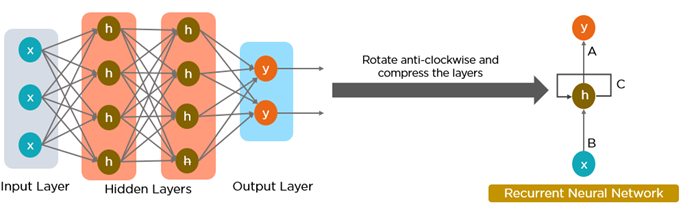
\includegraphics[width=15cm, height=7cm]{rnn1.png}
		\caption{Recurrent Neural Network Architecture}
		\label{figrnn1}
	\end{figure}
\end{center}


Fig. \ref{figrnn1}, shows hidden states of RNN at different time instances. These different time instances share the same parameters. The RNN is capable of handling data dependencies in the sequential data but has some issues like it may have a Vanishing and Exploding gradient problem. The hidden state in RNN has limited capability so, it is not able to handle data dependencies if data is separated by many time steps.
\subsection{Long Short-Term Memory (LSTM)}
The RNN can handle the dependency between the data if the two relevant data points are not far apart but if there is a long-term dependency between data then the RNN suffers from vanishing gradient problem. The LSTM model is a variant of the RNN model and it can handle this long-term dependency problem.
\par As shown in Fig. \ref{lstm}, in addition to hidden state $h_t$ the LSTM has one more state called cell state $C_t$. The hidden state is short-term memory and the cell state is long-term memory. The cell state $C_t$ is like a convey belt that passes information from the current time step to the next time step. Unlike RNN the LSTM does not remember all previous information. It only remembers relevant information, passes only necessary information to the next time step, and takes only fruitful information from the input using three gates viz. forget gate, output gate, and input gate. In Fig. \ref{lstm}, The forget gate $f_t$ govern by the following equation, decides which part of the input cell state $C_{t-1}$ is forgeted.
\begin{equation}
	\quad f_t = \sigma(W_{f} \cdot [h_{t-1},x_t] + b_{f})
\end{equation}
The input gate decides this part of the input added to the cell state $C_{t}$, govern by following equations as $i_t\ast \tilde{C_t}$.
\begin{equation}
	\quad i_t = \sigma(W_{i} \cdot [h_{t-1},x_t] + b_{i})
\end{equation}
\begin{equation}
	\quad \tilde{C_t}= \tanh(W_{c} \cdot [h_{t-1},x_t] + b_{c})
\end{equation}
The cell state ${C_t}$ is computed as 
\begin{equation}
	\quad \tilde{C_t}= f_t\ast {C_{t-1}} + i_t\ast \tilde{C_t}
\end{equation}
The output $h_t$ is computed as
\begin{equation}
	\quad {o_t}= \sigma(W_{o} \cdot [h_{t-1},x_t] + b_{o})
\end{equation}
\begin{equation}
	\quad {h_t}= {o_t}\ast  \tanh(C_t)
\end{equation}
In the above equations, $W$ is the weight vector and $b$ is the bais of the respective gate.



\begin{center}
	\begin{figure}[!htbp]
		\centering
		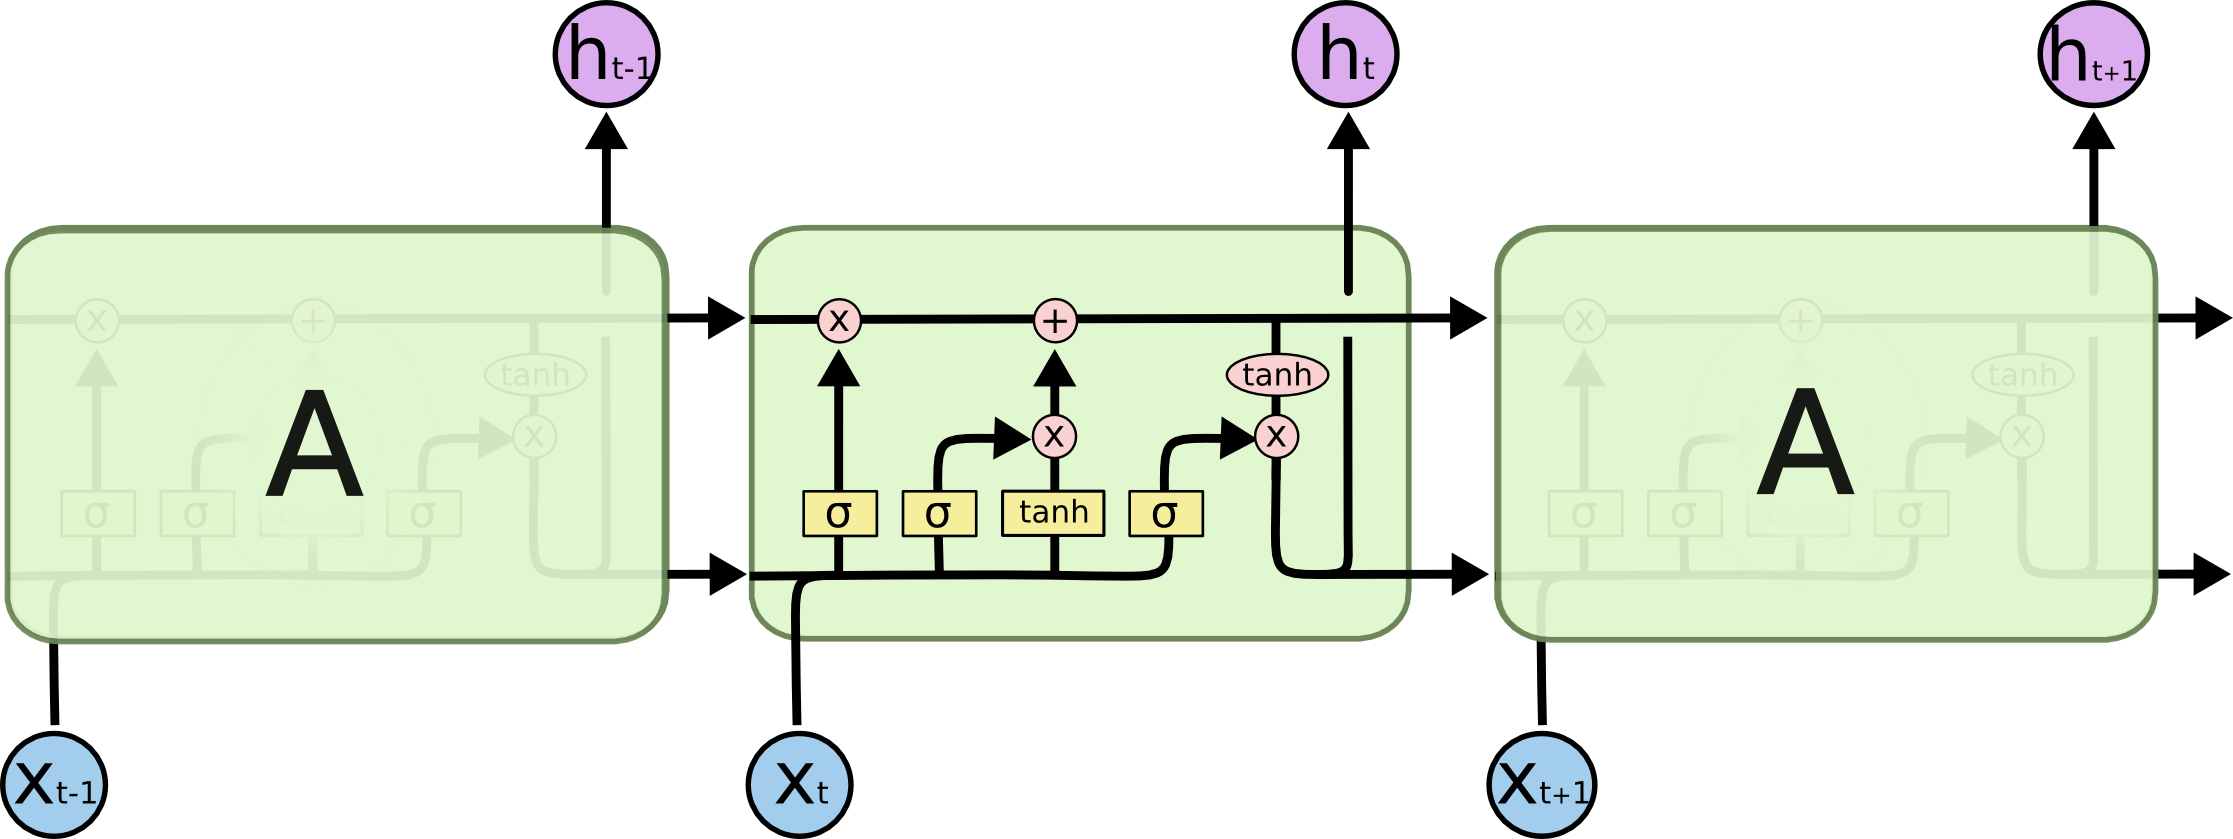
\includegraphics[width=12cm, height=5cm]{lstm.png}
		\caption{LSTM architechture}
		\label{lstm}
	\end{figure}
\end{center}


\subsection{GRU}
\par Gated Recurrent Unit (GRU) is introduced in \cite{cho2014learning}, like LSTM it is also a type of RNN that addresses the vanishing gradient problem. Like LSTM it also has gates but only two gates instead of three gates in LSTM. These two gates are namely the reset gate and the update gate. Unlike LSTM there is only one state. It has only a hidden state no cell state. The GRU architecture is less complex compared to LSTM. It is computationally less complex compared to LSTM. LSTM can capture better long-term dependency. The reset gate equation is as follows. The vector $r_t$ depends on the previous hidden state $h_{t-a}$ and current input $x_t$
\begin{equation}
	\quad r_t = \sigma(W_{r} \cdot [h_{t-1},x_t] + b_{r})
\end{equation}
The update gate is as follows. 
\begin{equation}
	\quad u_t = \sigma(W_{u} \cdot [h_{t-1},x_t] + b_{u})
\end{equation} 
The equation for candidate hidden state $\tilde{h_t}$ is as follows. where $\odot$ is elementwise multiplication.  
\begin{equation}
	\quad \tilde{h_t}= \tanh(W_{h} \cdot [r_t\odot h_{t-1},x_t] + b_{h})
\end{equation}
The current hidden state ${h_t}$ is computed as follows.
\begin{equation}
	\quad {h_t}= (1-u_t) \odot h_{t-1} + u_t \odot \tilde{h_t}
\end{equation}

\subsection{Convolutional Neural Network}
The Convolutional Neural Network (CNN) is introduced in \cite{krizhevsky2012imagenet}. It is a deep neural network and consists of a series of layers of type convolutional layer, pooling layer, and fully connected layer. It is typically useful for visual tasks but it also has utility in other types of data like numeric and text data \cite{chakole2021convolutional}. The main operation is convolution operation which is useful for feature extraction. The major role of the pooling layer is dimensionality reduction. After a series of convolution and pooling layers a fully connected layer is connected to map extracted features to the desired output.

\subsection{Transformer}
Unlike LSTM, GRU, and other primitive RNN-based models that rely on sequential processing, the Transformer on the other hand adopts a localized and hierarchical processing approach inspired by Convolutional Neural Networks (CNN). The key innovation lies in the integration of attention-based mechanisms which allows parallel computation and makes it possible to capture long-range dependencies thereby making it more efficient as shown in Fig. \ref{transformer}.
\begin{center}
	\begin{figure}[!htbp]
		\centering
		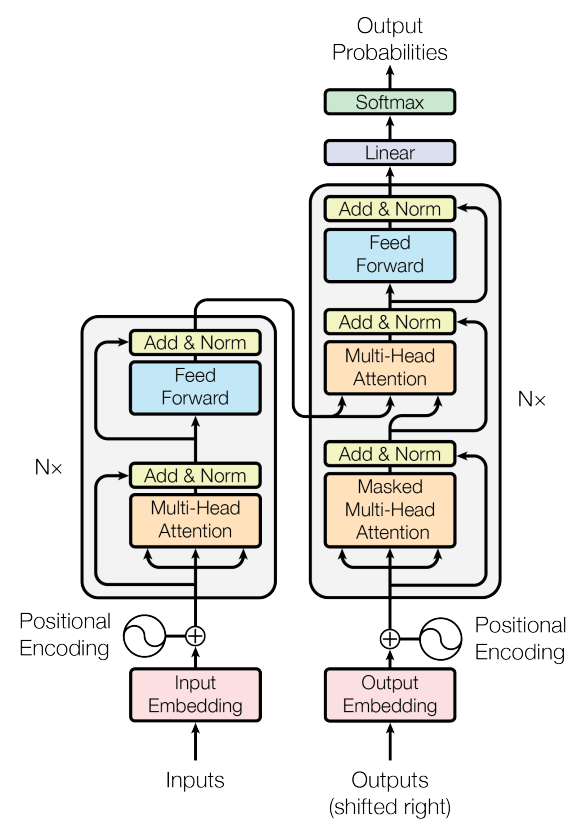
\includegraphics[width=10cm, height=12cm]{transformer.png}
		\caption{The Transformer - model architecture}
		\label{transformer}
	\end{figure}
\end{center}
\begin{itemize}
	\item \textbf{Attention Mechanism}\\
	It is a mechanism that assigns different levels of importance to different parts of the input sequence, enabling the model to selectively focus on different parts of the input sequence when producing an output, thereby selecting the most relevant information \cite{bahdanau2014neural}. Attention mechanisms are classified into self-attention, multi-head attention, and local attention, each offering different benefits and trade-offs.
	
	\item \textbf{Transformer}\\
	Introduced in the paper \cite{vaswani2017attention}, Transformer architecture is the fundamental building block of Large Language Models (LLMs). The self-attention mechanism helps to capture long-distance context so that the sequence of the hidden states also attends to itself. A Transformer model can be classified into three categories: Encoders, Decoders, and Encoder-decoder models\cite{sutskever2014sequence}. The attention mechanism involves three sets of matrices: query(Q), key(K), and value(V). These matrices are derived from the input sequence.
	\begin{itemize}
		\item \textbf{Query (Q)}\\
		The query vector represents the element that is currently being focused on for the given context. In the context of self-attention mechanisms, it's the vector of target input for which the attention weights are obtained. By transforming the word representation using the query matrix, the system generates a query vector that will be used to compare against other words in the sentence.	\\
		$q_{i}=W_{q}x_{i}$,  where $x_{i}$ represents the input query vector at position $i$, $q_{i}$ represents the projected query vector at position $i$,$W_{q}$ represents the weight matrix used for the query projection.
		\item \textbf{Value (V)}\\
		The key matrix is used to create key vectors for all words in the sentence. These key vectors help the system measure the relevance or similarity between the target word (using the query vector) and other words in the sentence. A higher similarity score between the query vector and a key vector indicates a stronger relationship between the corresponding words.\\
		$v_{i}=W_{v}x_{i}$
		\item \textbf{Key (K)}\\The value matrix generates value vectors for all words in the sentence. These vectors hold the contextual information of each word. After calculating the similarity scores using query and key vectors, the system computes a weighted sum of the value vectors. The weights for each value vector are determined by the similarity scores, ensuring that the final contextual representation is influenced more by relevant words.\\
		$k_{i}=W_{k}x_{i}$
		\item The encoding results in the word $C_i$, by applying attention mechanism to the projected vectors.	\\
		$r_{ij}=(q_{i}.k_{j})/\sqrt{d}$\\\\
		$a_{ij}=e^{r_{ij}}/(\sum_{k}^{} e^{r_{ik}})$\\\\
		$c_{i}=\sum_{j}^{} a_{ij}.V_{j}$\\
		where, $d$ represents the dimensionality of the key vectors.
	\end{itemize}
	Self-attention is only one component of the Transformer model. Each Transformer layer consists of several sub-layers. At each Transformer layer, self-attention is applied first. The output of the attention module is fed through feedforward layers, where the same feedforward weight matrices are applied independently at each position. A nonlinear activation function typically ReLU, is applied after the first feedforward layer.
	\begin{itemize}
		\item Inputs: Input sequential data tokens are converted to numerical representations called "input embeddings" using a dictionary-like mapping, where similar words have similar vector representations.
		
		\item Positional Encoding: Encodes the order of words in the input sequence as numbers, enabling the model to understand sentence structure.\\
		$P E_{(pos,2i)}=\sin (\frac{pos}{10000^{2i/{d_{model}}}})$\\
		
		$P E_{(pos,2i+1)}=\cos (\frac{pos}{10000^{2i/{d_{model}}}})$\\
		where:
		\begin{itemize}
			\item $pos$ is the position of the token in the sequence
			\item $i$ is the dimension index within positional encoding.
			\item $d_{model}$ is the dimension of the model
		\end{itemize}
		
		
		
		\item Encoder: Processes the input text through multiple self-attention layers, generating hidden states that capture meaning and context at different abstraction levels.
		
		\item Outputs (shifted right): During training, the decoder predicts the next word based on previous words, achieved by shifting the output sequence.
		\item Output Embeddings: Similar to input embeddings, representing predicted words as numbers and applying positional encoding.
		\item Loss Function: Measures the difference between predictions and actual text, guiding parameter adjustments to improve accuracy.
		\item Decoder: Uses the encoded input and positional information to generate natural language text, similar to the encoder, using multiple layers.
		\item Linear Layer and Softmax: Transforms output embeddings back to the original input space and generates a probability distribution for each possible output token.
	\end{itemize}
\end{itemize}

\section{Proposed Models}
The daily price sequence of the Aluminium on the London Metal Exchange (LME) is the time series data.  Researchers used this price data to generate derived spatial features to train machine learning models. Some of them used this price data to generate temporal features to train time series based models for price prediction. As the metal price data is time series data, the use of a time series or sequential model for the prediction of metal price looks promising. 
\par The main problem with the sequential data is to identify which part of the sequence is relevant for current prediction. The deep learning model LSTM has the capability to capture the relevant information from the input sequence using selective read, write, and forget. The encoder-decoder model is suitable for sequential data but it is not capable of handling long-term dependency. The attention mechanism resolved this problem but as the attention-based encoder-decoder model is based on RNN, we have to provide input in a sequential manner. This is the hurdle for parallelism. 
\par The Transformer is a recent deep learning algorithm that has shown outstanding performance on the sequential data in the NLP domain. The Transformer is based on the Attention mechanism to capture relevant information of the given sequential data. The Transformer model is also based on the encoder-decoder model but it doesn't use RNN. Instead it uses self-attention encoding and decoding. In Transformer parallel processing is possible need to provide data in a sequential manner.
\par In this research work our main objective is the identify the relevant parts of the input sequence for optimal prediction of the metal price using the state-of-the-art deep learning framework Transformer. We aim to explore the Transformer abilty of paying attention on relavant part of the data to predict the future price of the non-ferrous metals. Also, our another objective is to comapare the performance of the Transformer based model with other prominent deep learning approaches like LSTM, GRU, CNN for non-ferrous metals price prediction. We have proposed a Transformer-based deep learning model for metal price prediction as shown in Fig \ref{figpp}. 
\par As in Fig \ref{figpp}, firstly we perform data preprocessing like handling NaN values. Then we transform the raw data into label data for supervise learning problem. Input feature is eight days close price $[d_{t-7},d_{t-6},d_{t-5},d_{t-4},d_{t-3},d_{t-2},d_{t-1},d_{t}]$ and expected output is close price for $t+1$ day $d_{t+1}$. No need for input embedding as data is already a vector of real numbers. We have to perform positional encoding to preserve the sequence information. This input is passed to the encoder of the Transformer, where self-attention is performed to obtain revised context vector embedding. Encoder operations are performed more than one time and then the final output of the encoder is passed to the decoder of the Transformer.The decoder performs its operation in an iterative manner including self-attention to generate the output i.e. closing price for the $t+1$ day based on the input previous eight days' close price of the metal.
\par The Fig. \ref{fighm} is a heatmap. A heatmap is used for showing the corelation between the two features. We wanted to understand the experimental data. We initially thought that there should be a relation between the non-ferrous metal price and the coal price, so we checked it by performing the correlation test between the metal price and the coal price. Our results of correlation indicate that there is no correlation between the coal price and the metal price. A heatmap is a matrix of features. The value of the correlation coefficient ranges from -1 to +1. From Fig. \ref{fighm}, we can conclude that the price of the four experimental metals is correlated to each other.

\begin{center}
	\begin{figure}[!htbp]
		\centering
		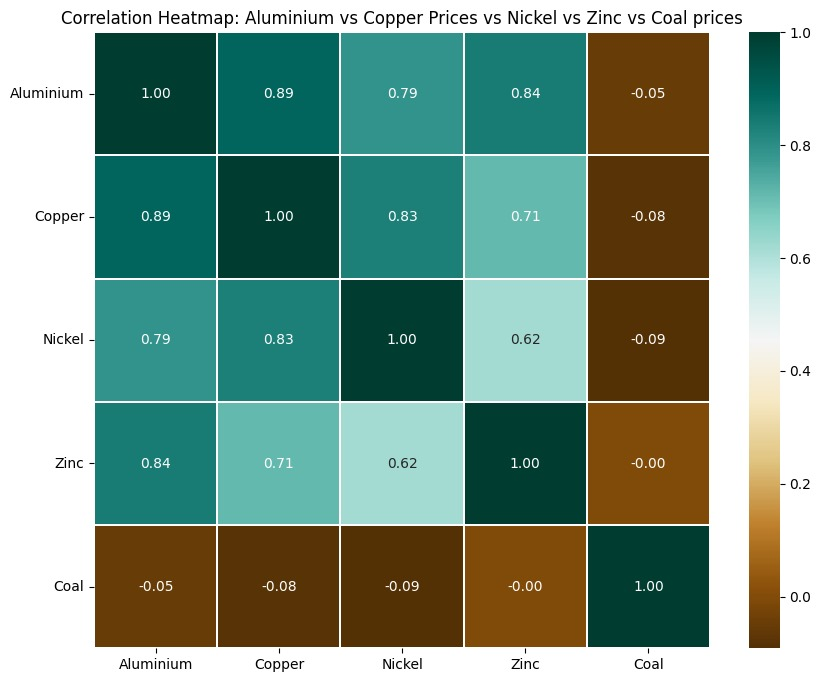
\includegraphics[width=12cm, height=10cm]{heatmap.jpeg}
		\caption{HeatMap}
		\label{fighm}
	\end{figure}
\end{center}

\begin{center}
	\begin{figure}[!htbp]
		\centering
		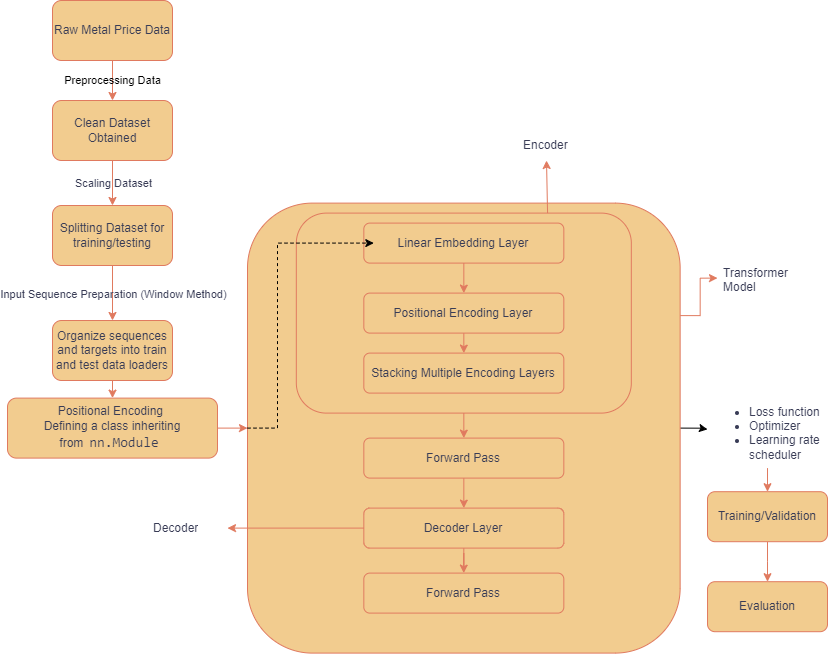
\includegraphics[width=15cm, height=14cm]{ps.png}
		\caption{Proposed System}
		\label{figpp}
	\end{figure}
\end{center}



\section{Experimentation}

\subsection{Experimental Data}
The global pricing of base metals such as Aluminium, Copper, Zinc, and others is determined by the London Metal Exchange (LME), a renowned commodities exchange based in London, United Kingdom, established in 1877. The LME facilitates futures and options trading for a variety of base and precious metals. Traders have the opportunity to engage in trading contracts for future delivery or options on a daily, weekly, and monthly basis. The prices of Aluminium, Copper, Zinc, and Nickel are denoted in US dollars per metric ton on the LME platform. In this work, we are interested in predicting the future price of the non-ferrous metal. Table \ref{tab1} shows the experimental data used in this work. We got this data from LME.


\begin{table}[!htbp]
	\begin{center}
		\begin{tabular}{ p{1.5cm}p{1cm}p{2cm}p{2cm}p{2cm}  } \hline
			
			Stock Name &Time &Total Period &Training Period &Testing Period\\ \hline \hline \\
			\multirow{2}{*}{Aluminium}&Start & 2008-01-02  &2008-01-02  &2020-12-02 \\
			&End & 2024-03-01 &2020-12-02 &2024-03-01\\ \hline\\
			\multirow{2}{*}{Copper}&Start & 2008-01-02  &2008-01-02  &2020-12-02 \\
			&End & 2024-03-01 &2020-12-02 &2024-03-01\\ \hline\\
			\multirow{2}{*}{Zinc}&Start & 2008-01-02  &2008-01-02  &2020-12-02 \\
			&End & 2024-03-01 &2020-12-02 &2024-03-01\\ \hline\\
			\multirow{2}{*}{Nickel}&Start & 2008-01-02  &2008-01-02  &2020-12-02 \\
			&End & 2024-03-01 &2020-12-02 &2024-03-01\\ \hline \hline
		\end{tabular}
		\caption{Experimental Data of Metal Prices from LME} \label{tab1}
	\end{center}
\end{table}
Figure \ref{fig:A}, Figure \ref{fig:Co}, Figure \ref{fig:Z}, Figure \ref{fig:N} are the plots of the experimental datasets used in this work, it show the daily closing price of the stock.
\begin{center}
	\begin{figure}[!htbp]
		\centering
		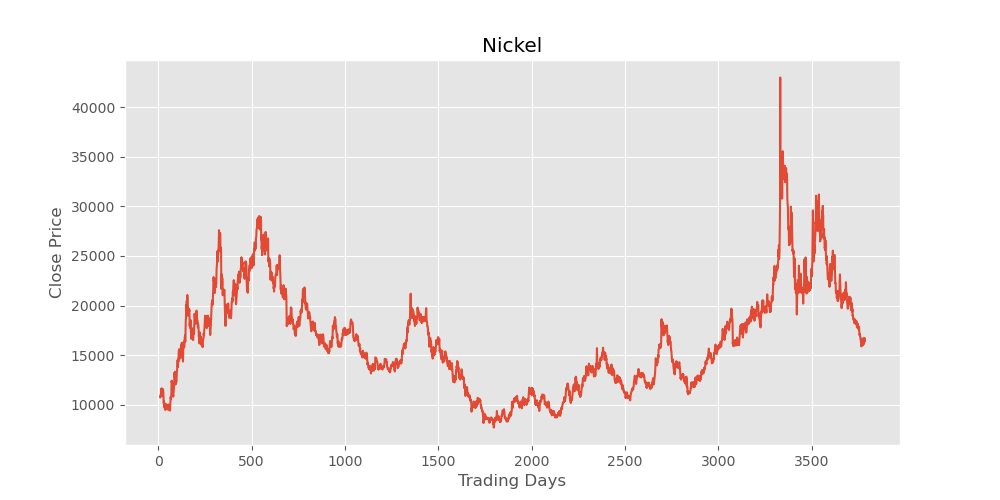
\includegraphics[width=15cm, height=7cm]{N.png}
		\caption{Daily close price series for Nickel.}
		\label{fig:N}
	\end{figure}
\end{center}

\begin{center}
	\begin{figure}[!htbp]
		\centering
		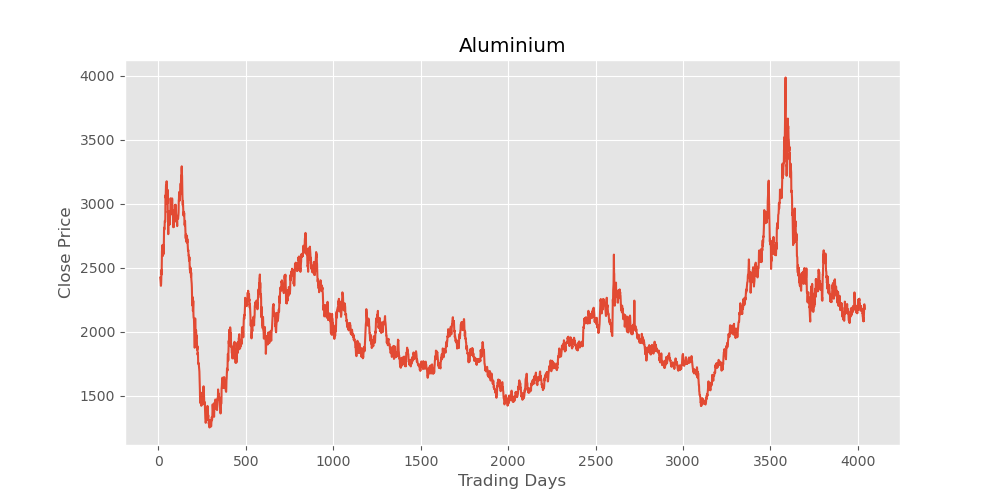
\includegraphics[width=15cm, height=7cm]{A.png}
		\caption{Daily close price series for Aluminium.}
		\label{fig:A}
	\end{figure}
\end{center}

\begin{center}
	\begin{figure}[!htbp]
		\centering
		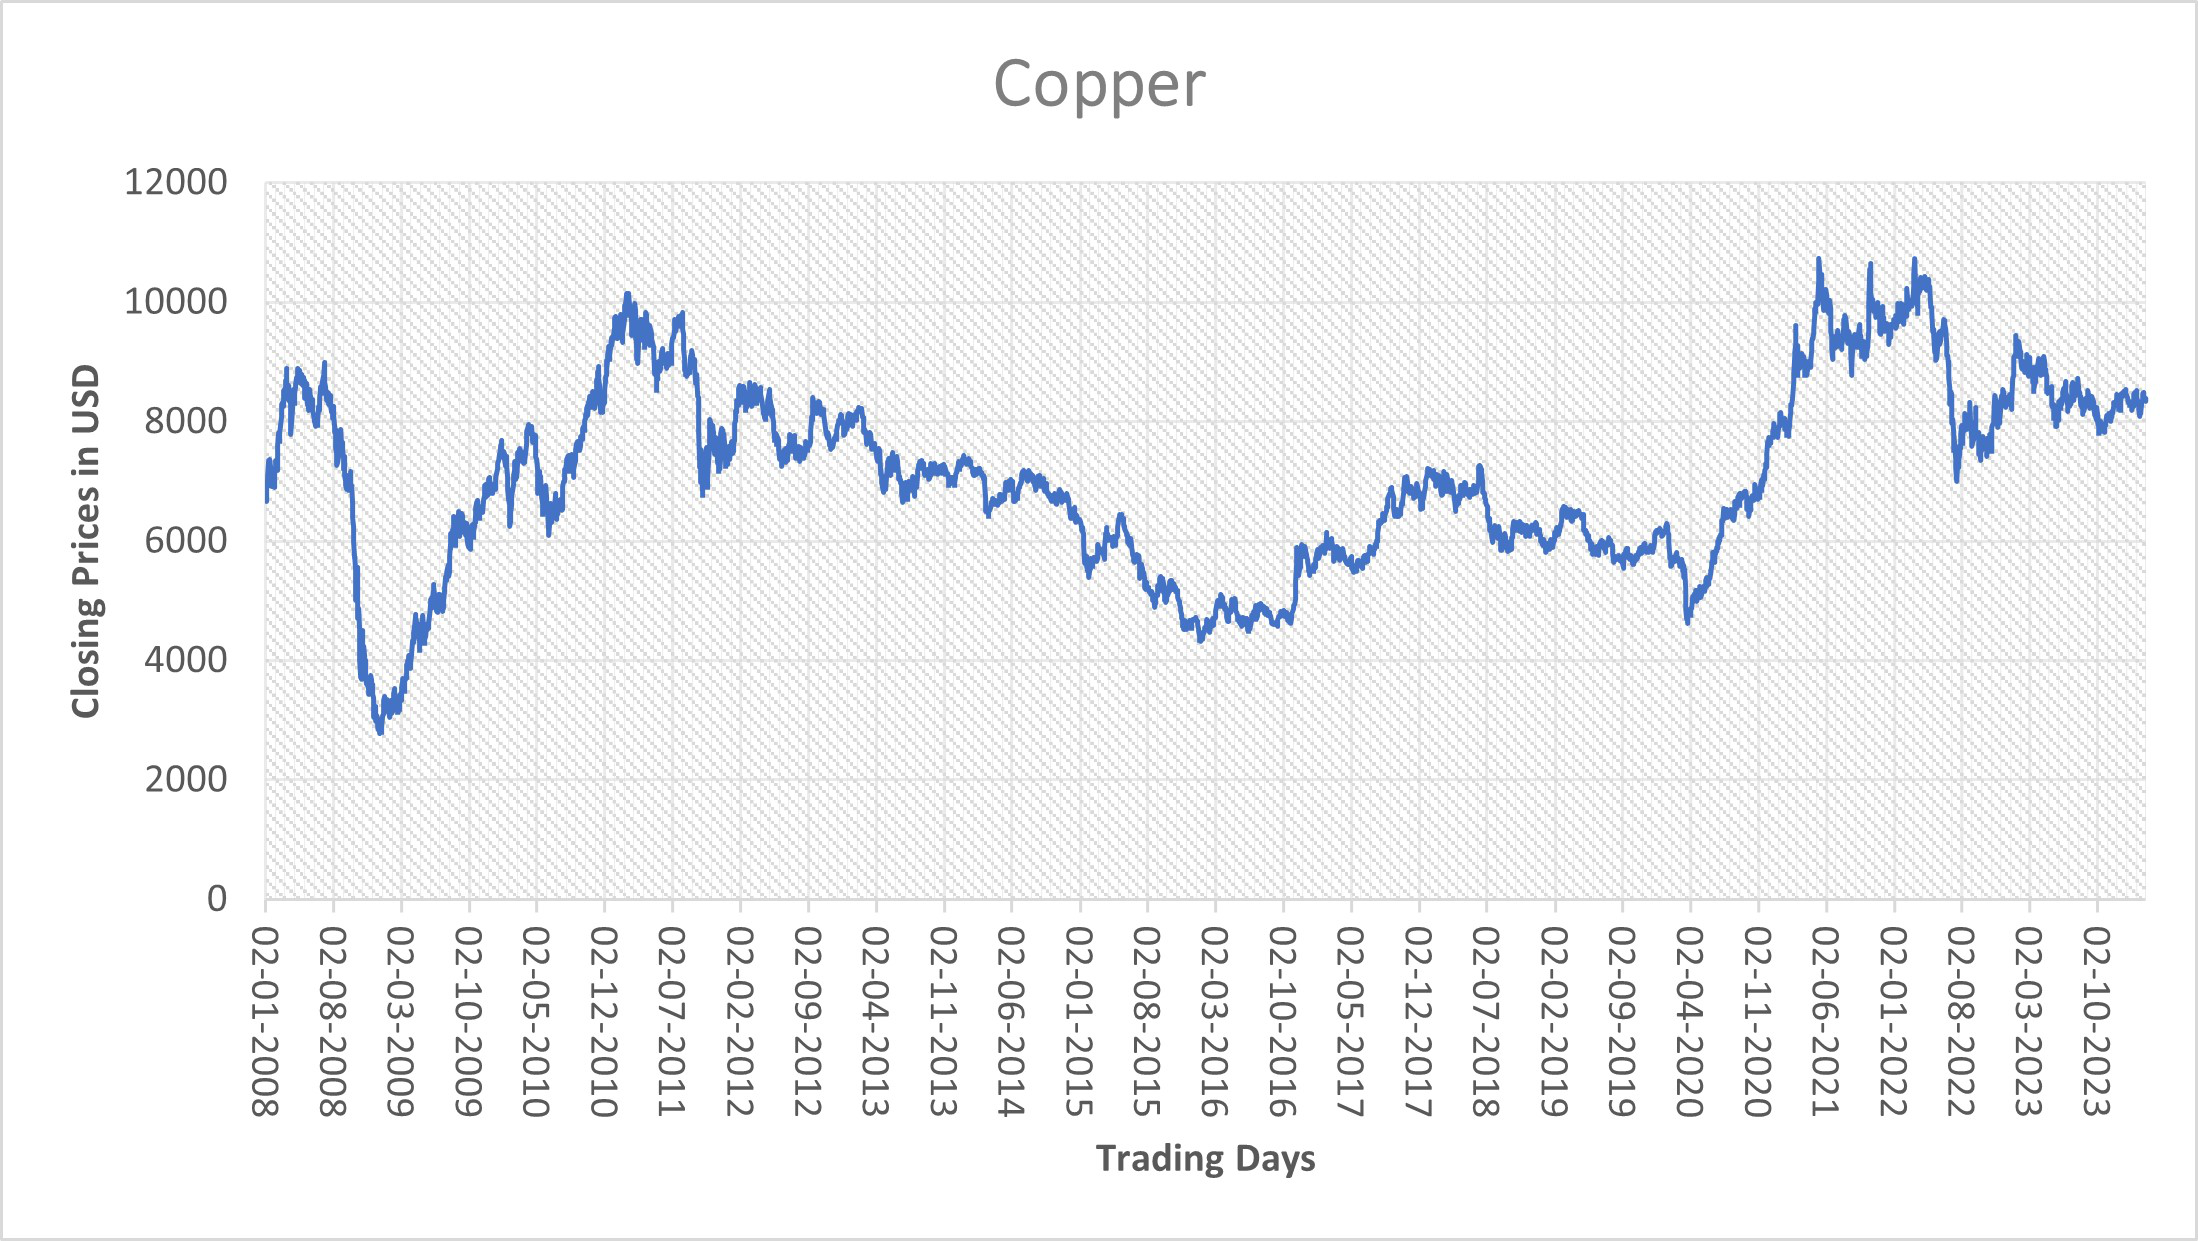
\includegraphics[width=15cm, height=7cm]{Co.png}
		\caption{Daily close price series for Copper.}
		\label{fig:Co}
	\end{figure}
\end{center}

\begin{center}
	\begin{figure}[!htbp]
		\centering
		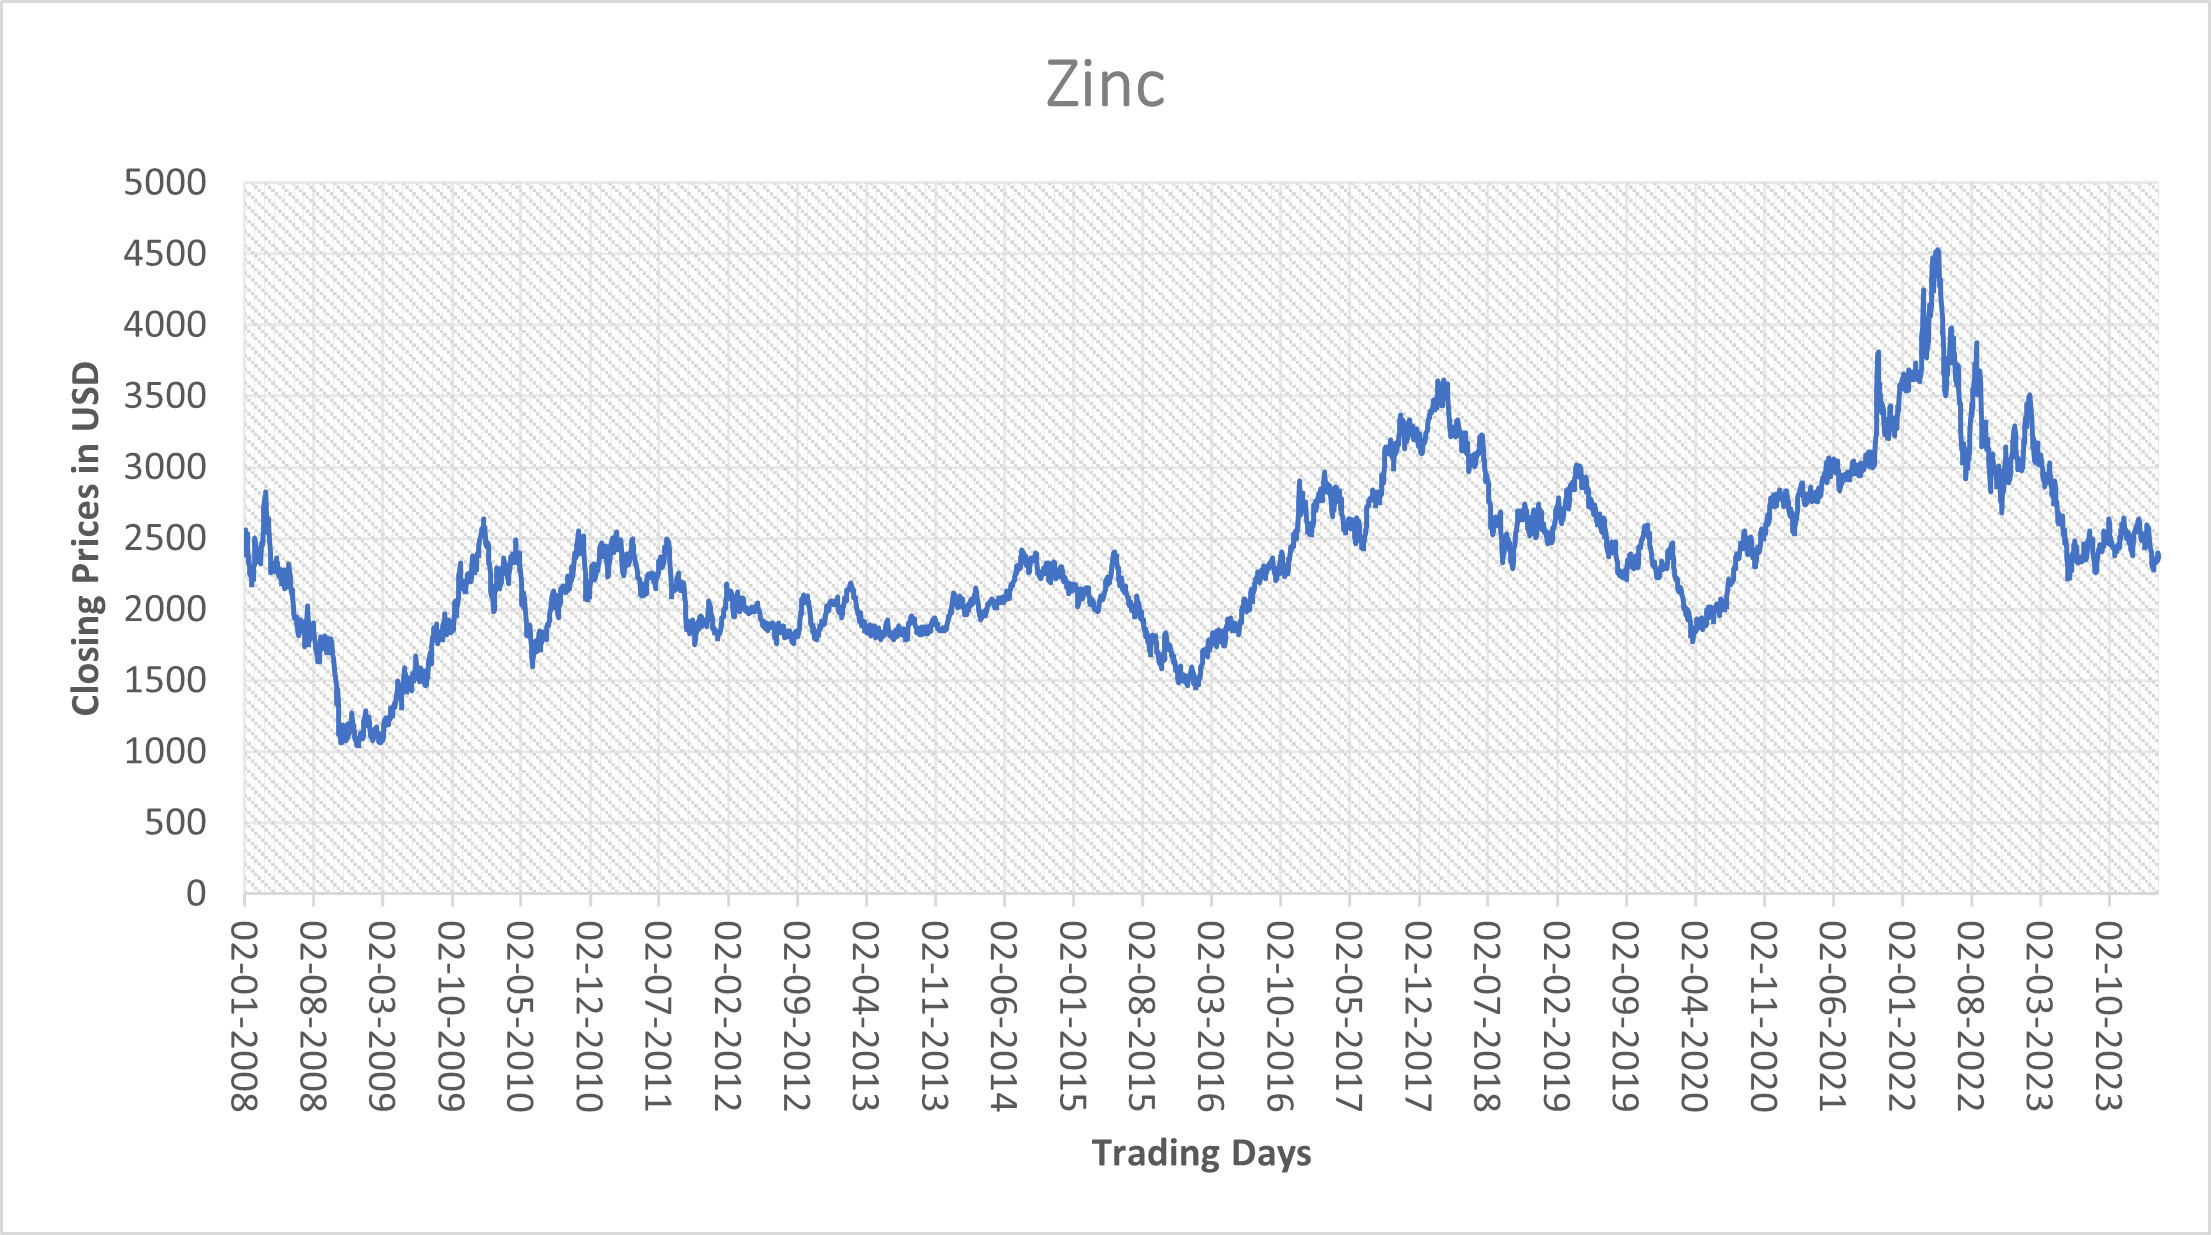
\includegraphics[width=15cm, height=7cm]{Z.png}
		\caption{Daily close price series for Zinc.}
		\label{fig:Z}
	\end{figure}
\end{center}

\subsection{Performance Evalution Measures}
Performance evaluation metrics are essential for assessing the effectiveness of models in various tasks, including regression problems. Mean Squared Error (MSE), Mean Absolute Error (MAE), and Mean Absolute Percentage Error (MAPE) are commonly used metrics for evaluating the performance of regression models.

\subsubsection{Mean Squared Error(MSE)}
A lower MSE indicates better model performance, and the metric is sensitive to outliers due to the squaring of errors.
\begin{equation}
	MSE = \frac{1}{n} \sum_{i=1}^{n} (y_i - \hat{y}_i)^2
\end{equation}

where:
\begin{align*}
	n & : \text{Number of data points} \\
	y_i & : \text{Actual value of the i-th data point} \\
	\hat{y}_i & : \text{Predicted value of the i-th data point}
\end{align*}

\subsubsection{Mean Absolute Error(MAE)}
Like MSE, a lower MAE indicates better model performance, and the metric is less sensitive to outliers than MSE.
\begin{equation}
	\text{MAE} = \frac{1}{n} \sum_{i=1}^{n} \lvert y_i - \hat{y}_i \rvert
\end{equation}

\subsubsection{Mean Absolute Percentage Error (MAPE)}
MAPE provides a percentage measure of the average relative error. A lower MAPE indicates better model performance, but it is sensitive to zero values in the actual data.
\begin{equation}
	MAPE = \frac{1}{n} \sum_{i=1}^{n} \left| \frac{y_i - \hat{y}_i}{y_i} \right| \times 100\%
\end{equation}

where:
\begin{align*}
	n & : \text{Number of data points} \\
	y_i & : \text{Actual value of the i-th data point} \\
	\hat{y}_i & : \text{Predicted value of the i-th data point}
\end{align*}

\section{Experimental Results}
We experimented with the proposed model on four metals viz Aluminium, Copper, Zink, and Nickel. We also compared the performance of the proposed model with the state-of-the-art deep learning methods LSTM, GRU, and CNN. All models are trained and tested on the same dataset for fair comparison. The performance of the models is compared using the performance evaluation measures discussed in Section 5.2.
\par The experimental results of all models including the proposed model for a dataset of Aluminium, Copper, Zink, and Nickel the Table \ref{tab2},  \ref{tab3},  \ref{tab4}, and  \ref{tab5} respectively. The proposed Transformer-based model outperformed all four baseline models on all four metals datasets with regards to MSE, MAE, and MAPE. Figure \ref{figr1} compares the performance of all experimental models in terms of MSE. This Figure clearly indicates that the proposed model is superior to all other models. 

\begin{table}[!htbp]
	\begin{center}
		\begin{tabular}{ p{3cm}|p{3cm}|p{3cm}|p{3cm} } \hline
			
			\textbf{Model}& \textbf{MSE}&\textbf{MAE}&\textbf{MAPE}\\ \hline 
			LSTM&0.000608 &0.01684& 2.0161\\ \hline 
			LSTM Multivariate&0.000771 &0.02039&1.9768\\ \hline
			GRU&0.000774 &0.01748&1.6579\\ \hline
			GRU Multivariate&0.000829 &0.02220&2.0703\\ \hline
			Transformer&0.000389 &0.01607 &1.5471\\ \hline
		\end{tabular}
		\caption{Performance of the five models including proposed Transformer based model on testing dataset of Aluminium} \label{tab2}
	\end{center}
\end{table}



\begin{table}[!htbp]
	\begin{center}
		\begin{tabular}{ p{3cm}|p{3cm}|p{3cm}|p{3cm} } \hline
			
			\textbf{Model}& \textbf{MSE}&\textbf{MAE}&\textbf{MAPE}\\ \hline 
			LSTM&0.000491 &0.021854& 1.9440\\ \hline 
			LSTM Multivariate&0.001229 &0.017297&2.5990\\ \hline
			GRU&0.001138 &0.030629&2.6538\\ \hline
			GRU Multivariate&0.000496 &0.018520&1.6476\\ \hline
			Transformer&0.000593 &0.01761&1.6861\\ \hline
		\end{tabular}
		\caption{Performance of the five models including proposed Transformer based model on testing dataset of Copper} \label{tab3}
	\end{center}
\end{table}

\begin{table}[!htbp]
	\begin{center}
		\begin{tabular}{ p{3cm}|p{3cm}|p{3cm}|p{3cm} } \hline
			
			\textbf{Model}& \textbf{MSE}&\textbf{MAE}&\textbf{MAPE}\\ \hline 
			LSTM&0.000611 &0.019248& 2.0187\\ \hline 
			LSTM Multivariate&0.000621 &0.018777&2.0797\\ \hline
			GRU&0.001019 &0.016316&1.8464\\ \hline
			GRU Multivariate&0.000789 &0.021309&2.0525\\ \hline
			Transformer&0.000486 &0.016580&1.9840\\ \hline
		\end{tabular}
		\caption{Performance of the five models including proposed Transformer based model on testing dataset of Zinc} \label{tab4}
	\end{center}
\end{table}

\begin{table}[!htbp]
	\begin{center}
		\begin{tabular}{ p{3cm}|p{3cm}|p{3cm}|p{3cm} } \hline
			\textbf{Model}& \textbf{MSE}&\textbf{MAE}&\textbf{MAPE}\\ \hline 
			LSTM&0.000959 &0.017043& 2.6024\\ \hline 
			LSTM Multivariate&0.000813 &0.016965&2.5462\\ \hline
			GRU&0.000703 &0.015500&2.3311\\ \hline
			GRU Multivariate&0.000721 &0.016193&2.3563\\ \hline
			Transformer&0.0006365 &0.019031&2.1635\\ \hline
		\end{tabular}
		\caption{Performance of the five models including proposed Transformer based model on testing dataset of Nickel} \label{tab5}
	\end{center}
\end{table}

\begin{center}
	\begin{figure}[!htbp]
		\centering
		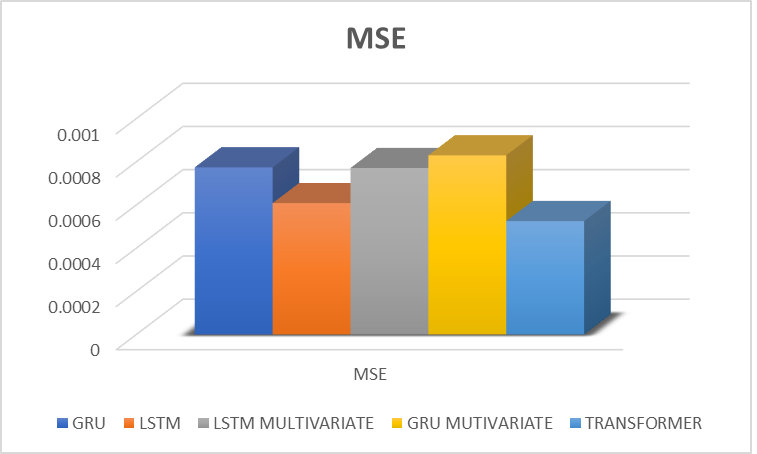
\includegraphics[width=15cm, height=7cm]{r1.png}
		\caption{MSE of the five models including proposed Transformer based model on testing dataset of Aluminium}
		\label{figr1}
	\end{figure}
\end{center}

\section{Conclusion}
Handling the long-term dependency on sequential data like metal price time series data is a problem of interest for industry and academia. LSTM results are better compared to RNN up to a certain extent. Recently deep learning model Transformer has shown significant performance improvement. We proposed a model based on a Transformer to predict the future price of the metal using historical and current price time series data of the metal. Our experimental results on datasets from LME conclude that the proposed model outperformed the baseline deep learning methods for sequential data. Till now Transformer for metal price prediction has not been studied. The main contribution of this research work is twofold. First, the use of a Transformer for metal price prediction. Second, is a comparison with the current state of art deep learning base model for sequential data. In the future, we would like to explore the Large Language Model for metal price prediction.  
\par Our experiment on the four datasets indicates that the Transformer based model outperformed the LSTM and GRU-based models to predict future metal price in terms of MSE, MAE, and MAPE. 

\bibliography{sample} 
\bibliographystyle{plain}
\end{document} 